\section{Исследовательский раздел} 
В данном разделе...

\subsection{Технические характеристики системы}
Исследование проводилось на персональном компьютере со следующими характеристиками:

\begin{itemize}
\item процессор Intel(R) Core(TM) i7-10510U CPU @ 1.80GHz,
\item операционная система Linux (дистрибутив Manjaro Linux, версия ядра Linux 5.13.19-2-MANJARO, архитектура x86-64),
\item 16 Гб оперативной памяти.
\end{itemize}

Вывод разработанных компонентов сохранялся в отдельные текстовые файлы и в дальнейшем, для определения разницы, анализировался с использованием утилиты sdiff.

Для определения того, какие процессы задействуют директорию или файл, использовалась утилита lsof.

\subsection{6 итераций вывода информации о процессах реального времени с разницей в 10 секунд при воспроизведении аудио с использованием MPlayer}
Перед началом исследований было проверено, что аудиофайл не задействован никакими другими процессами, как это показано на рисунке \ref{fig:emptylsof}.

\begin{figure}[H]
	\centering
	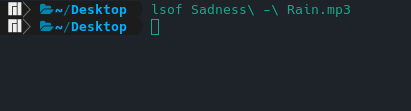
\includegraphics[scale=1]{img/emptylsof.png}
	\caption{Подтверждение того, что файл не задействован никакими другими процессами.}
	\label{fig:emptylsof}
\end{figure}

При запуске проигрывания с использованием MPlayer, утилита lsof указывает на то, что файл используется процессом с именем mplayer (рисунок \ref{fig:mplayerlsof}).

\begin{figure}[H]
	\centering
	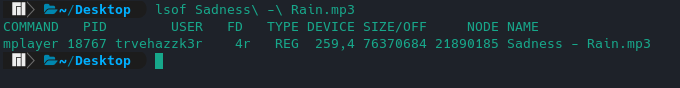
\includegraphics[scale=0.8]{img/mplayerlsof.png}
	\caption{Результат запуска утилиты lsof при воспроизведении файла с использованием Mplayer.}
	\label{fig:mplayerlsof}
\end{figure}

При проведении исследования, первые 10 секунд композиция не запускается. Это связано с тем, что перерывы между получением информации о процессах в модуле заданы данным интервалом времени. Таким образом можно будет наблюдать возможное появление нового процесса, либо динамику изменения полей отдельных task\_struct, отнесенных к задачам реального времени.

В силу того, что файл вывода содержит 1666 строк, его представление здесь нецелесообразно. При анализе результатов было обнаружено, что среди процессов, отнесенных к задачам реального времени, отсутствует процесс с идентификационным номером 18767. Причем, при использовании утилиты pstree у данного процесса обнаруживается лишь один потомок, у которого более нет потомков. Важно отметить также тот факт, что завершение потомка влечет за собой и завершение родительского процесса.

\subsection{6 итераций вывода информации о процессах реального времени с разницей в 10 секунд при воспроизведении аудио с использованием VLC Media Player}
Для достоверности результатов также будет попытка использовать VLC Media Player. Данное исследование проводилось также, как и предыдущее.

\begin{figure}[H]
	\centering
	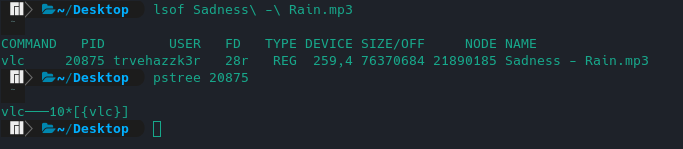
\includegraphics[scale=0.8]{img/vlclsof.png}
	\caption{Результат запуска утилит lsof и pstree при воспроизведении файла с использованием VLC Media Player.}
	\label{fig:vlclsof}
\end{figure}

В силу того, что файл вывода содержит 1666 строк, его представление здесь нецелесообразно. При анализе результатов было обнаружено отсутствие среди проанализированных процессов задачи с идентификационным номером 20875.

\textbf{Таким образом для дальнейшей работы потребуется проверить, совпадут ли данные выводы при использовании функции task\_is\_realtime, которая определяет принадлежность процесса к задачам реального времени по политике планировщика.}

\subsection{6 итераций вывода информации с использованием функции task\_is\_realtime с разницей в 10 секунд при воспроизведении аудио с использованием MPlayer и VLC Media Player}
Исходный код загружаемого модуля был изменен, как это указано в листинге \ref{code:newModule}.

\begin{code}
	\captionof{listing}{Измененная часть вывода в модуле.}
	\label{code:newModule}
	\inputminted
	[
	frame=single,
	framerule=0.5pt,
	framesep=20pt,
	fontsize=\small,
	tabsize=4,
	linenos,
	numbersep=5pt,
	xleftmargin=10pt,
	firstline=63,
	lastline=78,
	breaklines=true
	]
	{text}
	{code/mdWithTaskIsRealtime.c}
\end{code}

При анализе результатов было обнаружено отсутствие среди приведенных процессов задачи с идентификационным номером, совпадающим с номером процессов, отвечающих за воспроизведение ни в случае использования MPlayer, ни в случае использования VLC Media Player.

\textbf{Таким образом для дальнейшей работы потребуется убрать условие выборки определения принадлежности процесса к задачам реального времени и проанализировать поля структуры task\_struct. }

\subsection{6 итераций вывода информации о всех процессах в системе с разницей в 10 секунд при воспроизведении аудио с использованием VLC Media Player. }
Исходный код загружаемого модуля был изменен, как это указано в листинге \ref{code:newNewModule}.

\begin{code}
	\captionof{listing}{Измененная часть вывода в модуле.}
	\label{code:newNewModule}
	\inputminted
	[
	frame=single,
	framerule=0.5pt,
	framesep=20pt,
	fontsize=\small,
	tabsize=4,
	linenos,
	numbersep=5pt,
	xleftmargin=10pt,
	firstline=61,
	lastline=79,
	breaklines=true
	]
	{text}
	{../../src/md.c}
\end{code}

При проведении исследования производились две остановки воспроизведения на 5 секунде и 15 секунде. Время каждой остановки составляло 6--7 секунд. Процесс, отвечающий за воспроизведение, имел идентификационный номер 7702. В итоге, в выводе была получена информация, предоставленная в листинге \ref{code:firstVlcLog}.

\begin{code}
	\captionof{listing}{Информация о процессе vlc.}
	\label{code:firstVlcLog}
	\inputminted
	[
	frame=single,
	framerule=0.5pt,
	framesep=20pt,
	fontsize=\small,
	tabsize=4,
	linenos,
	numbersep=5pt,
	xleftmargin=10pt,
	breaklines=true
	]
	{text}
	{code/firstVlcLog.txt}
\end{code}

Видно, что со временем динамика отсутствует. Таким образом, можно сделать вывод, что, либо процесс был определен неверно, либо сам VLC Media Player обладает более сложным поведением.

\subsection{6 итераций вывода информации о всех процессах в системе с разницей в 10 секунд при воспроизведении аудио с использованием MPlayer. }
При воспроизведении остановок не производилось. Процесс, отвечающий за воспроизведение, имел идентификационный номер 9126. При этом он имел дочерний процесс 9127. В итоге была получена информация, предоставленная в листинге \ref{code:firstMplayerLog}.

\begin{code}
	\captionof{listing}{Информация о процессе mplayer.}
	\label{code:firstVlcLog}
	\inputminted
	[
	frame=single,
	framerule=0.5pt,
	framesep=20pt,
	fontsize=\small,
	tabsize=4,
	linenos,
	numbersep=5pt,
	xleftmargin=10pt,
	breaklines=true
	]
	{text}
	{code/firstMplayerLog.txt}
\end{code}

Из предоставленной информации можно видеть, что в структуре изменяются поля delay, utime и stime. Причем значение поля static\_prio равняется значению поля normal\_prio, что означает, что процесс не относится к задаче реального времени.

В динамике заметно возрастание времени, проведенного в режиме пользователя и затраченное на запуск команд (utime), а также времени процессора, затраченного на выполнение системных вызовов при исполнении процесса (stime). В среднем за каждые 10 секунд utime увеличивался на 105 340 32 тика, в то время как stime в среднем увеличивался на 4 438 620.5 тика, что на $\approx$ 58 \% меньше.

Важно отметить, что никакой информации о процессе с номером 9127 обнаружено не было.

В сложившейся ситуации также было проверено, что MPlayer является клиентом PulseAudio (многофункциональный звуковой сервер, предназначенный для работы в качестве прослойки между приложениями и аппаратными устройствами, либо ALSA (Advanced Linux Sound Architecture) или OSS (Open Sound System)), с использованием утилиты pacmd, в которой была вызвана команда list-clients. Результат вывода предоставлен в листинге \ref{code:pacmd}. Идентификационный номер также совпал.

\begin{code}
	\captionof{listing}{Информация, полученная с использованием утилиты pacmd.}
	\label{code:firstVlcLog}
	\inputminted
	[
	frame=single,
	framerule=0.5pt,
	framesep=20pt,
	fontsize=\small,
	tabsize=4,
	linenos,
	numbersep=5pt,
	xleftmargin=10pt,
	breaklines=true
	]
	{text}
	{code/pacmd.txt}
\end{code}

Полученные результаты говорят о том, что сами программы воспроизведения не создают процессы, относящиеся к задачам реального времени. В источнике \cite{hackerNews} говорится о том, что планирование SCHED\_FIFO может быть использовано лишь для потоков ввода-вывода. Таким образом, только потоки ввода-вывода PulseAudio выполняются в режиме реального времени, а управляющий поток, так называемый MainLoop, обычно остается обычным потоком.

Из предоставленной информации становится ясно, что потребуется провести анализ потоков, создаваемых при воспроизведении аудио.

\subsection{Исследование потоков, создаваемых PulseAudio. }
При запуске воспроизведения команда ps может позволить получить информацию о потоках приложения, что предоставлено на рисунке \ref{fig:psThreads}.

\begin{figure}[H]
	\centering
	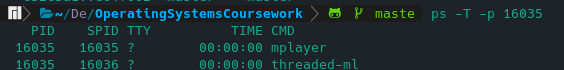
\includegraphics[scale=0.8]{img/psThreads.png}
	\caption{Содержание журнала ядра. }
	\label{fig:psThreads}
\end{figure}

На предоставленном изображении \ref{fig:psThreads} SPID -- это идентификационный номер потока. Таким образом, потребуется получить некоторую информацию о потоке, которая может быть предоставлена утилитой top.

\subsection*{Вывод}
В разделе...
